\chapter{Results}

\section{Single language}
All experiments depicted in this section are based on a configuration shown in section
~\ref{sec:basic_params}. In Table~\ref{tab:universal} we show our baseline results
for a subset of the UD languages (due to limited computational resources we were
not able to train models for all of them). The results are compared to
SyntaxNet~\cite{andor_globally_2016} and ParseySaurus~\cite{alberti_parsey_saurus_2017},
both from Google. The ParseySaurus is based on SyntaxNet, and uses characters
as input, while the original SyntaxNet uses word embeddings. Both are transition-based,
and need no external POS tagger.
It is worth noting that SyntaxNet has different hyperparameter configuration
for each language, while our parser uses the same configuration across all languages.

\begin{table}[!htbp]
  \centering
  \begin{tabular}{l l | l l | l l | l l}
    language & \#sentences & \multicolumn{2}{c|}{Ours} & \multicolumn{2}{c|}{SyntaxNet} & \multicolumn{2}{c}{ParseySaurus} \\ \hline
    & & UAS & LAS & UAS & LAS & UAS & LAS\\ \hline
    Czech & 87 913 & \textbf{91.41} & \textbf{88.18} & 89.47 & 85.93 & 89.09 & 84.99 \\
    Polish & 8 227 & 90.26 & 85.32 & 88.30 & 82.71 & \textbf{91.86} & \textbf{87.49}\\
    Russian & 5 030 & 83.29 & 79.22 & 81.75 & 77.71 & \textbf{84.27} & \textbf{80.65} \\
    German & 15 892 & 82.67 & 76.51 & 79.73 & 74.07 & \textbf{84.12} & \textbf{79.05}\\
    English & 16 622 & 87.44 & 83.94 & 84.79 & 80.38 & \textbf{87.86} & \textbf{84.45}\\ 
    French & 16 448 & \textbf{87.25} & \textbf{83.50} & 84.68 & 81.05 & 86.61 & 83.1\\
    Ancient Greek & 25 251 & \textbf{78.96} & \textbf{72.36} & 68.98 & 62.07 & 73.85 & 68.1
  \end{tabular}
  \caption{Baseline results of models trained on single languages from
    UD v1.3. Our models use only the orthographic representation of
    tokenized words during inference and works without a separate POS tagger.}
  \label{tab:universal}
\end{table}

In the following sections we will show impact of different network parameters
on the result.

\subsection{Impact of \emph{reader} and \emph{predictor}}
We first inspect the impact of different \emph{reader} and \emph{predictor}
settings.
\begin{table}[!htbp]
  \centering
  \label{tab:results}
  \begin{tabular}{l|cc|cc|cc|}
    training inputs & \multicolumn{2}{c|}{Czech} & \multicolumn{2}{c|}{English} & \multicolumn{2}{c|}{Polish} \\
    & UAS & LAS & UAS & LAS & UAS & LAS \\ 
    \multicolumn{7}{c}{Gold POS tags} \\  \hline
    base word & 
    \textbf{91.7} & \textbf{88} & 
    \textbf{88.6} & 85.1 & 
    \textbf{93.4} & \textbf{89.3} \\
    \multicolumn{7}{c}{Predicted POS tags or no POS tags} \\ \hline
    words & 
    82.4 & 72.1 &
    81.9 & 74.7 & 
    74.6 & 61.6  \\
    chars, soft att. & 
    \textbf{90.1} & 85.7 & % results/inprogress/lab110-01/dependency_norec_smaller_cz/pretraining_best.zip
    86.5 & 82.1 & % results/inprogress/sonata2/dep_en/pretraining_best.zip
    89.1 & 82.5 \\ %results/inprogress/lab110-11/dep_pl_lessclip/pretraining_best.zip
    chars, tags, soft att. & 
    89.6 & 82.8 & % lab110-02 results/inprogress/lab110-02/dependency_norec_smaller_cz_tags/pretraining_best.zip
    86.2 & 81.3 & % results/inprogress/sonata1/dep_en_tags/pretraining_best.zip
    90.4 & 83.9 \\ % results/inprogress/lab110-03/dep_cpw_opt_no_r_tags/pretraining_best.zip
    chars, tags, hard att. & 
    \textbf{90.1} & \textbf{86.7} & % results/inprogress/lab110-01/dependency_norec_smaller_cz_tags_l0_hard_restart/pretraining_best.zip
    \textbf{87.6} & \textbf{83.6} & % sonata2 local_storage/dependency_norec_spbest_en_tags_l0_hard/pretraining_best.zip
    \textbf{91.3} & \textbf{86} \\ % results/inprogress/lab110-17/dependency_norec_smaller_pl_tags_l0_hard/pretraining_best.zip
  \end{tabular}
  \caption{Model performance on selected languages and different training inputs. Experiments were run on \textbf{UD v 1.2}} 
\end{table}

In the upper part "Gold POS tags" we show a favorable situation when we have access
to gold pos tag (approved by a human). The inputs are base words embedded in a vector 
(we replace the \emph{reader} subnetwork with simple, learnable table lookup).
This setting allowed us to obtain best results (especially for Polish) but
gold pos tag are not available in a real-word setting so this result is noted just
as a upper band of the model perfromance.

The "words" and "chars, soft att." settings don't use a \emph{predictor}. Using just words
as inputs (embedded in the same manner as base word) gives worst results. This is
easy to predict because most words in the dataset occurs only once and so the
network doesn't have a clue about role of most of the words.
Instead, using character-level input allows us to obtain much better results, especially
because in morphosyntactically rich languages the word spelling catches many
word features that can be used in deducing the pos tag information.

The result of adding a \emph{predictor} depends on the attention type used.
Used with soft attention it decreased the results in Czech and English, but increased
in Polish. When hard attention is used it can obtain the best results in all cases.
The intuition behind these results is that with hard attention the labeller only
sees annotation of the chosen head, and the error is backpropagated only to this
element. On the other hand with soft attention the head annotation refers
to many incorrect words introducing more noise. Additionally the soft attention labeller
error is backpropagated through all words, which can introduce even more noise on the neural weights.


\subsection{Impact of decoding algorithm}

In the Table~\ref{tab:edmonts_baseline} we show the comparison of greedy and
Chu-Liu-Edmonds decoding algorithms.

\begin{table}[!htbp]
  \centering
  \begin{tabular}{l | c c}
    language & Greedy UAS & Edmonds UAS \\ \hline
      Czech & \textbf{91.41} & 91.40 \\
      Polish &  \textbf{90.26} & 90.17 \\
      Russian & \textbf{83.29} & 83.23 \\
      German &  \textbf{82.67} & 82.66 \\
      English & \textbf{87.44} & 87.41 \\
      French &  \textbf{87.25} & 87.18 \\
      Ancient Greek & \textbf{78.96} & 78.92
  \end{tabular}
  \caption{The comparison of greedy and edmonts decoding algorithms}
  \label{tab:edmonts_baseline}
\end{table}

\begin{figure}[!htbp]
  \centering
  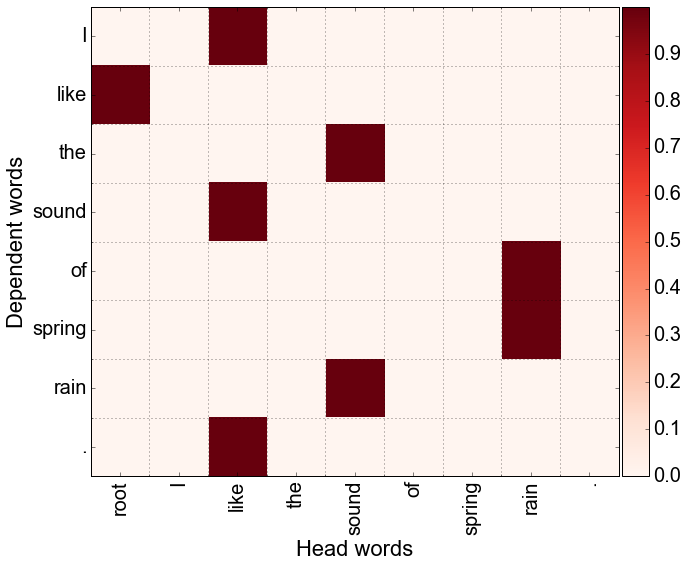
\includegraphics[width=0.6\linewidth]{img/examples/cle/attention.png}
  \caption{A typical scorer output showing probabilities assigned for head-word location.} 
  \label{fig:attention}
\end{figure}

Counter intuitively the CLE algorithm makes the decoding results slightly worse.
We have investigated this and the problem lies in the confidence of the
\emph{scorer} predictions which are very sharp (see Figure~\ref{fig:attention}).
Additionally non-top scores are very noisy and do not reflect  meaningful alternatives,
thus CLE algorithm finds a cycle it is very probable that it will break it
in wrong place, creating another error. The example of such behaviour is depicted
in Figure~\ref{fig:cle}.

\begin{figure}[!htbp]
  \centering
  \resizebox{\textwidth}{!}{
    \import{img/examples/cle/}{cle.pdf_tex}
  }
  \caption{Dependency tree for sentence "What to do to advert the threat lurking on ice?".
    The dashed-dotted (zagrożenia\txtrightarrow lodzie), dotted (czyhającego\txtrightarrow uniknąć)
    and dashed (zagrożenia\txtrightarrow uniknąć) arcs denote, respectively greedy, CLE, and groundtruth decodings.
    The greedy decoder produced the incorrect dependency zagrożenia\txtrightarrow lodzie instead of
    zagrożenia\txtrightarrow uniknąć which created a cycle zagrożenia\txtrightarrow lodzie\txtrightarrow czychającego\txtrightarrow zagrożenia.
    However, the CLE algorithm replaced the good connection
    czyhającego\txtrightarrow zagrożenia with czyhającego\txtrightarrow uniknąć
    which removed the cycle but introduced a new error.} 
  \label{fig:cle}
\end{figure}

We tried to counteract this by using label-smoothing regularization (LSR)
\cite{szegedy_rethinking_2015}.
It is a very simple method of regularization which changes 1-hot vector encoding
of groundtruth data to some other distribution which have effect of lowering overconfidence
of the network. In our case we soften the head position groundtruth vector by
giving the proper head 51\% probability and uniformly distribute the rest 49\%
among other words. Unfortunately this method did not improve the overall CLE algorithm
score.

\subsection{Recurrent state size}
We have also investigated the impact of the \emph{tagger} recurrent state size.
It is desirable to have as small recurrent state size as possible because this
part of the network is activated as many times as there are words in the sentence,
making it a big performance factor.

\begin{table}[!htbp]
    \centering
    \begin{tabular}{l c c c c}
        Language & \% of recurrent state size & UAS & LAS \\ \hline
        \multirow{3}{*}{Polish}& 100\% & 90.26 & 85.32 \\
        & 50\% & \textbf{90.54} & \textbf{85.64} \\
        & 25\% & 89.07 & 82.80 \\ \hline
        \multirow{3}{*}{Czech}& 100\% & \textbf{91.41} & \textbf{88.18}\\
        & 50\% & 89.98 & 85.92\\
        & 25\% & 85.56 & 79.16\\ \hline% ale tutaj to malo epok bylo
    \end{tabular}
    \label{tab:birnn_single_size}
    \caption{Impact of the \emph{tagger} recurrent state size on the performance.
    We report this value as percent of baseline rnn size.}
\end{table}

We can see that in small dataset language like Polish there is not a big difference
between base and 50\% base, whereas in Czech the performance drop is significant.
Because we want to use the same architecture for every language the original 548
units recurrent state size is optimal.

\subsection{Word pieces model}
Following \cite{sennrich_subword_2015} we experimented with subword units.
Instead of using single characters as inputs we can find frequent common characters groups and
depict each word as combination of those units. Of course to be able to
present every word, each single letter also has to be treated as small subword unit. 
For example lets consider two polish words: \emph{lepszy} and \emph{najlepszy} (better, the best).
The \emph{naj} prefix in polish used with adjective means that it is in superlative degree,
so we can imagine that this letter composition is pretty common and thus will be
treated as subword unit. Then those two words will be shown to the network as
\emph{naj-l-e-p-s-z-y} and \emph{l-e-p-s-z-y} (- acting as subword delimiter).

Our word pieces model are obtained as follows:
first we compute word frequency dictionary  and initialize pieces dictionary with all characters in the dataset.
From frequency dictionary we take the most common character bigram and we treat it as new character and replace all previous occurrences
with this new unit. The number of such iterations is a parameter given by the user.
To convert word to pieces we use a greedy strategy. For word $w$ we find the longest
piece $p$ that is prefix of $w$. The next step takes $w$ suffix of size $\|w\| - \|p\|$.

\begin{table}[!htbp]
    \floatbox[{\capbeside\thisfloatsetup{capbesideposition={right,center},capbesidewidth=7cm}}]{figure}[\FBwidth]
    {\caption{Results on word pieces model. \#pieces denotes how many new
    multi-character tokens were used. To convert word to pieces we
    use a greedy algorithm in which we choose the longest piece that is equal
    to prefix of word.}
    \label{tab:word_pieces}}
{
    \begin{tabular}{c c c}
        \#pieces & UAS & LAS \\ \hline
        \multicolumn{3}{c}{Polish}\\
        25 & 90.29 &  84.91 \\
        50 & \textbf{90.40} &  \textbf{85.46}\\
        75 &  90.23 & 84.87\\
        100 & 89.97 & 84.44\\\hline
        \multicolumn{3}{c}{Czech}\\
        25 & 90.29 & 86.50\\
        50 & 90.03 & 86.08\\
        75 & 90.17 & 86.40\\
        100 & \textbf{90.84} & \textbf{87.31}
    \end{tabular}
}
\end{table}

In Table~\ref{tab:word_pieces} we have depicted the results of word pieces model
for different number od additional multi-character tokens. There is only minor
improvement for Polish while for Czech we have actually worse results. Additionally
this input model is not well suited for multilanguage parser, because the pieces
frequency is different for each language.

\section{Multilanguage training}
The main difference between multilanguage and single language configurations is
that we have to decide which parts of the network should have shared weights.
We tested it on 3 language pairs: Polish-Czech, Russian-Czech, Polish-Russian.
They all are from the same Slavic family, but Russian uses Cyrillic alphabet as
opposed to Latin script for Polish and Czech. The main advantage of Czech language
that made us choose it as auxiliary language is the quality and quantity of training data
- it is over 6 times bigger than Polish and Russian datasets combined.
The results of different sharing strategies are depicted in Table~\ref{tab:multi_baseline}.

\begin{table}[!htbp]
  \centering  
  \begin{tabular}{l | l l c c}
    Shared parts & Main lang & Aux lang & UAS & LAS \\ \hline
      - & Polish & - & 90.31 & 85.21 \\
    \emph{Parser} & Polish & Czech & 90.72 & 85.57 \\ % local_storage/multi/pl_cs_merge_generator
    \emph{Tagger, Parser} & Polish & Czech & 91.19 & 86.37 \\ % sonata2:  /pio/lscratch/1/i248100/pl_cs_unification_exclude_pos
    \emph{Tagger, POS Predictor, Parser} & Polish & Czech & 91.65 & 86.88 \\ % local_storage/dependency_pl_cs_new
    \emph{Reader, Tagger, POS Predictor, Parser} & Polish & Czech & \textbf{91.91} & \textbf{87.77} \\\hline % sonata1: /pio/lscratch/1/i248100/multi_pl_cs_different_eos_merge_all
    \emph{Parser} & Polish & Russian & 90.31 & 85.07 \\  % local_storage2/pl-ru-inc-generator
    \emph{Tagger, POS Predictor, Parser} & Polish & Russian &
    \textbf{91.34} & \textbf{86.36} \\ 
    \emph{Reader, Tagger, POS Predictor, Parser} & Polish & Russian & 89.16 & 82.94 \\  %  local_storage2/multi_pl_ru_different_eos_merge_all
\hline\hline % local_storage/multi/pl_ru_same_eos
    - & Russian & - & 83.43 & 79.24 \\
    \emph{Parser} & Russian & Czech & 83.15 & 78.69 \\  % sonata0: /pio/lscratch/1/i248100/ru-cs-parser
    \emph{Tagger, POS Predictor, Parser} & Russian & Czech & 83.91 & 79.79 \\ %  local_storage/multi/ru_cs
    \emph{Reader, Tagger, POS Predictor, Parser} & Russian & Czech & \textbf{84.78} & \textbf{80.35} % sonata1:  /pio/lscratch/1/i248100/ru-cs-all
  \end{tabular}
  \label{tab:multi_baseline}
  \caption{Impact of parameter sharing strategies on main language parsing accuracy when multilingual training
    is used for additional supervision.}
\end{table}


Multilingual training (Table~\ref{tab:multi_baseline}) improves the performance on low-resource languages.
We observe that the optimal amount of parameter sharing depends on the similarity
between languages and corpus size – while it is beneficial to share all parameters of the
PL-CZ and RU-CZ parser, the PL-RU parser works best if the reader subnetworks are
separated. 

Similarly as in the single language configuration we have tested the impact of \emph{tagger}
recurrent state size on the results (see Table~\ref{tab:birnn_multi_size}).

\begin{table}[!htbp]
    \centering
    \begin{tabular}{l c c c}
        \% of recurrent state size & UAS & LAS \\ \hline 
        200\% & 91.45 & 86.36\\
        100\% & \textbf{91.65} & \textbf{86.88}\\
        50\% & 89.53 & 83.66\\
        25\% & 87.28 & 78.93
    \end{tabular}
    \label{tab:birnn_multi_size}
    \caption{Impact of the \emph{tagger} recurrent state size on the performance
    of multilanguage pl-cz model.
    We report this value as percent of baseline rnn size.}
\end{table}

The results are computed on best Polish-Czech model (with share all strategy). We can see
that the recurrent state size have similar behaviour as in the single language Czech model - 
the 50\% size has significant drop in the performance. It is worth noting that
increasing the size changes the result only slightly (and that they are actually worse).
This mean that chosen \emph{tagger} size is well-suited for both single and multi
language parsers.

\subsection{Polish-Polish multilang parser}
After investigating results of the parser (this problem applies to both single
and multi parser) we have found that if the \emph{tagger} assigns wrong POS tag to
a particular word it can mislead the scorer and labeller producing wrong parse tree.
In many cases after replacing wrong word with its synonym such that the \emph{tagger}
will assign the right POS tag - the tree becomes a valid parse. For an example see Figure~\ref{fig:pos_bad_good}.

\begin{figure}[htbp]
  \centering
  \resizebox{0.8\textwidth}{!}{
    {\Large
      \import{img/examples/pos/}{bogumil.pdf_tex}
    }
  }
  \\[5pt]
  \resizebox{0.8\textwidth}{!}{
    {\Large
      \import{img/examples/pos/}{michal.pdf_tex}
    }
  }
  \caption{In the upper panel the sentence "Bogumił felt silent so
    much that he almost stopped breathing." is incorrectly parsed.
    We attribute the error to the \emph{reader} or to the \emph{tagger} because the predicted POS
    tag for "Bogumił", a male given name, is wrong (VERB instead of
    NOUN). In the lower panel we replace "Bogumił" with the  more common "Michał" the network assigns
    a proper tag and the whole sentence becomes a valid parse tree.} 
  \label{fig:pos_bad_good}
\end{figure}

The prevent this behaviour on Polish language we have decided to use additional data
for training the \emph{predictor} subnetwork. We used the \emph{milionowy podkorpus} (milion subcorpus)
of the National Corpus of Polish Language \cite{przepiorkowski_nkjp_2012}. We converted
this data to UD conllu format by filling the dependency information with a blank values
and transoforming the polish-style POS tags to UD-style using conversion table provided
by UD authors.
Next we used our multilingual training procedure in which the first langauge was
a standard UD Polish dataset, and the second one was our converted polish subcorpus.
The difference with previous attempts is that we have to ignore loss on dependency head
$L_h$ and dependency label $L_l$ for the second language.\\
This model allowed us to obtain our best results: \textbf{\todotext{XX}\% UAS} and \textbf{\todotext{XX}\% LAS}.
